% !TeX encoding = ISO-8859-1
\chapter{Einleitung}
\label{chap:einleitung}

\begin{figure}[h]
	\centering
	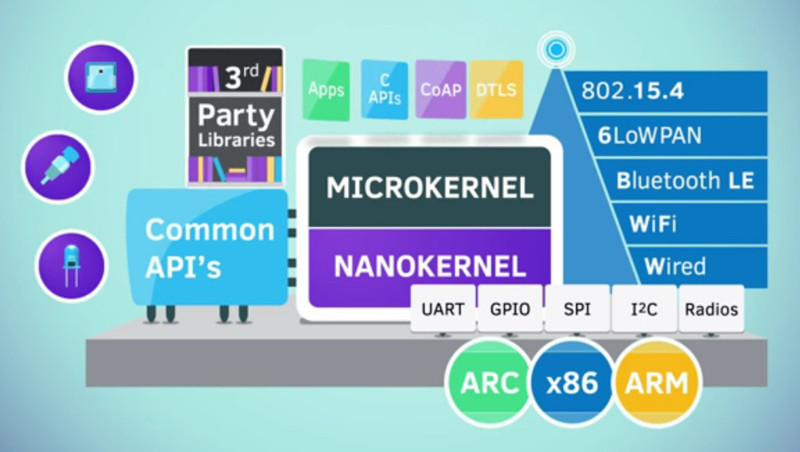
\includegraphics[width=0.7\linewidth]{bilder/zephyr_components.jpg}
	\caption{Komponenten und �bersicht �ber das Zephyr RTOS}
	\label{fig:components}
\end{figure}

In dieser Projektarbeit soll zuerst ein Vergleich der Eigenschaften �hnlicher
Betriebssysteme wie FreeRTOS, RIOT, Kontiki, usw. vor allem bez�glich der Unterst�tzung der
verschiedenen Netzwerkprotokolle gemacht werden. Im Fokus steht dabei das n
Zu Demonstrationszwecken soll am Schluss mit dem ausgew�hlten Board eine Demo-App entwickelt werden.

Die Ziele sind:

\begin{itemize}
	\item Einarbeitung in das Betriebssystem Zephyr.
	\item Erstellen einer Vergleichstabelle mit den wichtigsten Eigenschaften der verschiedenen
	RTOS.
	\item Evaluation geeigneter Boards f�r das Zephyr Betriebssystem f�r eine IoT
	\item Entwicklung einer Demonstrationsapplikation, basierend auf dem ausgew�hlten Board
\end{itemize}